\section{Multiplanet retrieval}
\label{sec:multis}

Similar to the single planet case, we compare the RNN-based detection algorithms with BLS in the task of retrieving planets with multiple transit signals. In this case we use Lilith data, which in some cases contain transit signals from different planets within the same light curve. Again we restrict both methods to only output three candidate detections per light curve, to save on computation time.

In this experiment we also include the TESS pipeline detections for the given data set. However, since a threshold has already been set on the pipeline detections, we only have limited data, and the PR-curve for the pipeline therefore cannot be drawn fully. For the pipeline's PR-curve shown in Figure \ref{fig:multi_pr}, we set a threshold on the SNR of the detections that are provided in the DV files. It can be seen from this figure, that the pipeline's PR-curve steadily decreases, suggesting that a high AP could be obtained if we had access to all the detections below the pre-set threshold. In contrast, the RNN-based algorithms drop down steeply. Nevertheless, the RNN-based methods seem to be able to maintain high precision for the detection of about 10\% of all the planets. BLS on the other hand, starts off with relatively low precision, but is able to retrieve far more of the total number of planets. In terms of average precision, it therefore outperformed the other methods. Figure \ref{fig:multi_transit} shows the detection results over the distribution of transit samples for different parameters. We can see that each method behaves similarly, but at different levels of performance. Table \ref{tab:multi_AnotB} presents the number of planets retrieved by each method, including the number of planets that were detected by one method and not by the other. Table \ref{tab:multi_AnotB} is provided to give a closer view on the ability of PTS-Fold and BLS-12h to retrieve multiple planets in a single light curve. From this table we can see that PTS-Fold is able to detect multiple planets in the same light curve, but there is room for improvement as compared to BLS-12h.

\begin{figure}
    \centering
    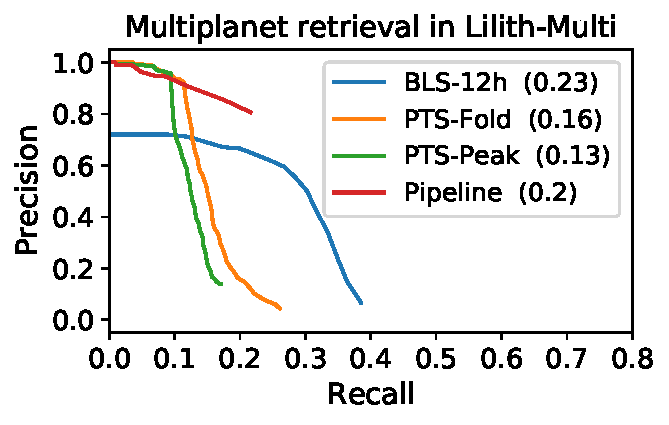
\includegraphics[width=0.35\linewidth]{Experiments/Figures/Multis/multi_pr.pdf}
    \caption{Precision-recall (PR) curves of different methods in the task of detecting repeating transit signals in light curves of Lilith-Multi. The PR-curve for the pipeline could not be drawn fully due to limited available data.}
    \label{fig:multi_pr}
\end{figure}

\begin{figure}
    \centering
    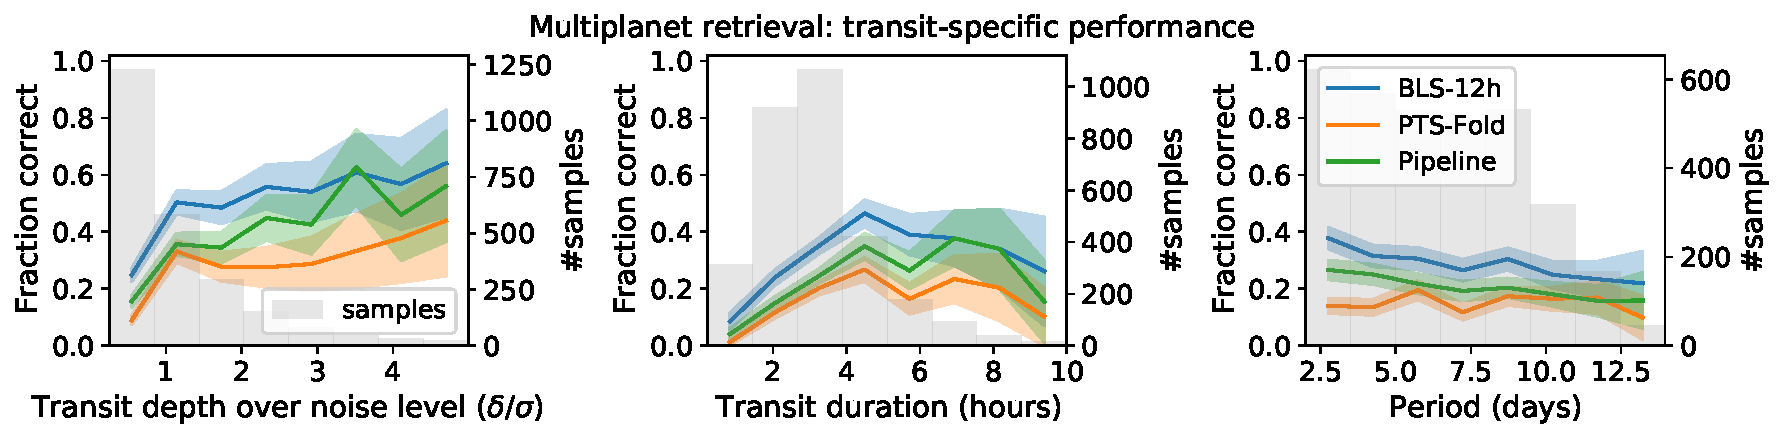
\includegraphics[width=\linewidth]{Experiments/Figures/Multis/multi_transit_specific.pdf}
    \caption{The ability of each method to retrieve planets in the given parameter ranges. A detection threshold is set closest to a corresponding detection precision of 0.5. Filled regions show the Wilson score interval \cite{wilson1927probable}, which approximates the 95\% confidence interval of the performance per bin.}
    \label{fig:multi_transit}
\end{figure}

\begin{table}[]
\label{tab:multi_AnotB}
\centering
\begin{tabular}{@{}lrlrlrl@{}}
\toprule
             & \multicolumn{2}{c}{PTS-Fold} & \multicolumn{2}{c}{BLS-12h} & \multicolumn{2}{c}{Pipeline} \\ \midrule
             & 493      & (1.00, 0.15)      & 993      & (1.00, 0.30)     & 710      & (1.00, 0.22)      \\
not PTS-Fold & -        &                   & 522      & (0.53, 0.16)     & 304      & (0.43, 0.09)      \\
not BLS-12h  & 22       & (0.04, 0.01)      & -        &                  & 46       & (0.06, 0.01)      \\
not Pipeline & 87       & (0.18, 0.03)      & 329      & (0.33, 0.10)     & -        &                   \\ \bottomrule
\end{tabular}
\caption{The absolute and relative number of correct detections in the task of retrieving planets with multiple transit signals, where the detection thresholds are set closest to a corresponding detection precision of 0.5. For the pipeline, the level of precision is in fact higher and the numbers presented here are relatively small, because we had no access to its lower confidence detections. The data contained a total of 3285 planets.}
\end{table}

\begin{table}[]
\label{tab:multi_numpl}
\centering
\begin{tabular}{@{}cccccc@{}}
\toprule
\multirow{2}{*}{\begin{tabular}[c]{@{}c@{}}\# planets\\ (\# light curves)\end{tabular}} & \multirow{2}{*}{Method} & \multicolumn{4}{c}{Detected} \\
                                                                    &          & 1   & 2  & 3 & 4 \\ \midrule
\multirow{2}{*}{\begin{tabular}[c]{@{}c@{}}1\\ (2130)\end{tabular}} & PTS-Fold & 371 &    &   &   \\
                                                                    & BLS-12h  & 666 &    &   &   \\ \cdashlinelr{1-6}
                                                    
\multirow{2}{*}{\begin{tabular}[c]{@{}c@{}}2\\ (474)\end{tabular}}  & PTS-Fold & 80  & 9  &   &   \\
                                                                    & BLS-12h  & 120 & 65 &   &   \\ \cdashlinelr{1-6}
                                                    
\multirow{2}{*}{\begin{tabular}[c]{@{}c@{}}3\\ (57)\end{tabular}}   & PTS-Fold & 13  & 5  & 0 &   \\
                                                                    & BLS-12h  & 8   & 20 & 6 &   \\ \cdashlinelr{1-6}
\multirow{2}{*}{\begin{tabular}[c]{@{}c@{}}4\\ (9)\end{tabular}}    & PTS-Fold & 1   & 0  & 0 & 0 \\
                                                                    & BLS-12h  & 4   & 2  & 1 & 0 \\ \bottomrule
\end{tabular}
\caption{The number of correctly detected planets per light curve with a given number of planets. For example, of the 57 light curves that contained 2 planets, PTS-Fold was able to retrieve 2 planets from 5 light curves, and only 1 planet from 13 light curves.  The detection threshold was set closest to a corresponding detection precision of 0.5.}
\end{table}
